\section{Labeling Guide Summary}\label{app:labels}
For each candidate, raters recorded:
\begin{itemize}
\item binding (Y/N/U);
\item whether the issue is a proof-system soundness bug;
\item the pattern (P1--P5, OTHER or NA);
\item C1--C3 individually (met, fails, unclear);
\item the effect, the unbound value and the intended policy (FULL tier);
\item confidence and notes.
\end{itemize}
The exclusions of Section~\ref{sec:definition} and the hard cases (attested
verification, signatures instead of proofs, multi-issue findings) follow the
guide in the artifact.

\section{No-Drop Admissibility Rules}\label{app:nodrop}
A candidate (withdrawn draft, unbound effect row, unconstrained statement row)
may be dropped \textbf{only} if: (1)~a final warning already reports the same
unbound value at the same primary location (file and function); (2)~the
review cited a concrete check (file:line) that binds the value on every path,
or showed that the attack only makes verification fail; (3)~a numbered
exclusion genuinely applies (quoted); or (4)~there is no concrete attacker
action (nothing the attacker changes while keeping a valid proof). Every other
reason is inadmissible, in particular: the consumer is not in the repository
(report at the circuit, guest or library); the attack needs another flaw as
well; the issue was folded into a finding whose primary location differs; it
is ``secondary'' to a bigger issue; it could not be traced to an effect
function although the proving component leaves a value the consumer acts on
unconstrained. Restored warnings use only paths and functions present in the
material, one per root cause, at the definition rather than per instantiated
copy.

\section{Scoring, Judge and Keep-Rule Counting}\label{app:count}
\para{Matching}
Strict: the warning's own file (basename) and function equal the ground-truth
location, case-insensitively and ignoring qualifiers, and the judge confirms
the mechanism. Loose: location only. Mechanism: any warning in the snapshot
that the judge accepts. A v1.1 amendment, adopted after round~1 and applied to
all tools, added the case-insensitive matcher and the mechanism level.

\para{Judge}
For each flaw the judge receives the ground-truth unbound value and effect
and, per candidate warning in the same snapshot, its pattern, effect,
unbound value and explanation, and answers yes or no. The prompt is frozen
(identified by its hash), the call has no tools, verdicts are cached per
(warning, flaw) pair, and a failed or non-binary answer aborts scoring rather
than counting as no.

\para{Keep rule}
For each configuration and run we count (a)~on every fixed-twin snapshot,
every \texttt{finding\_id} group whose locations are disjoint from all
locations the comparison configuration reports there, and (b)~every hard
negative flagged by the configuration but not by the comparison. The count is
averaged over the two runs and normalized per 10 of the 29 snapshots that
hold a fixed twin or hard negative; normalizing per unit (45) changes no
decision. Run-to-run noise is the same count between two runs of one
configuration. \emph{Correction after results:} for steps that change
Stage~A itself (knowledge), (a) had excluded new Stage~A findings and
undercounted; counting them raised knowledge from 0.52 to 3.97 per 10 and
turned a pass into a fail. No other decision changed.

\section{Execution-Loop Guards}\label{app:guards}
The first loop version produced a false pass: a scaffold deployed the
contract from the honest account, which made it the owner, and the owner's
repeated call to an owner-only mint looked like a replay. Six guards close
such loopholes. (O1)~Before a replay or same-sender success counts, the
honest call is retried from a fresh account; if access control rejects it,
the success is void. (O2)~Scaffolds deploy and grant roles from a separate
administrator. (O3)~A replay success requires a replay-key row, and the
second effect must touch that key. (O4)~A scaffold whose honest run fails a
check is redrafted. (O5)~The agent cannot give up before an LLM attempt, and
a give-up must cite an earlier outcome. (O6)~A mock verifier cannot tell
verifiers apart, so a success that swaps the verifier, proof type or key
counts only on the real verifier. Under a selection rule fixed in advance we
also compared discovery variants: an extractor-based coverage check found 70
rows the ledgers missed and judged none unbound, an execution sweep attacked
60 of 645 effect rows without success, and a depth pass into vendored
dependencies added one strict hit within run-to-run variance at 2.4 times the
cost. More reading did not help; the misses were judgments.

\section{Per-Item Results on Dev-v4}\label{app:items}
\begin{table*}[!htb]
\centering\footnotesize
\caption{Strict hits out of 2 runs per dev-v4 flaw. Layer: S Solidity, C
circuit, R Rust zkVM. ND: no-drop only; K: Stage A with knowledge; All: all
post steps. Recovery: how v4 obtains the hit.}
\setlength{\tabcolsep}{2.6pt}
\begin{tabular}{@{}llllrrrrrrl@{}}
\toprule
Item & Split & L & Pat. & v2 & ND & v4 & K & K+v4 & All & Recovery\\
\midrule
L001 & old-check & C & P2 & 1 & 1 & 1 & 0 & 0 & 1 & Stage A \\
L003 & old-tune & R & other & 0 & 0 & 0 & 0 & 0 & 0 & -- \\
L007 & v4-tune & S & P5 & 0 & 0 & 0 & 0 & 0 & 1 & -- \\
L008 & old-tune & R & P2 & 0 & 0 & 0 & 0 & 0 & 0 & -- \\
L010 & v4-tune & S & P1 & 0 & 0 & 0 & 1 & 1 & 0 & -- \\
L011 & old-tune & S & P1 & 1 & 1 & 1 & 2 & 2 & 1 & Stage A \\
L014 & old-tune & S & P2 & 2 & 2 & 2 & 2 & 2 & 2 & Stage A \\
L015 & v4-tune & S & P1 & 2 & 2 & 2 & 2 & 2 & 2 & Stage A \\
L017 & old-check & S & P1 & 2 & 2 & 2 & 2 & 2 & 2 & Stage A \\
L019 & old-check & S & P4 & 2 & 2 & 2 & 2 & 2 & 2 & Stage A \\
L020 & v4-tune & S & P3 & 0 & 0 & 1 & 0 & 0 & 0 & multi-loc.\ (placement) \\
L021 & v4-tune & S & P4 & 0 & 1 & 1 & 1 & 1 & 1 & no-drop (never reported) \\
L023 & old-check & S & P1 & 0 & 2 & 2 & 0 & 2 & 2 & no-drop (placement) \\
L030 & old-tune & R & P2 & 1 & 1 & 1 & 2 & 2 & 2 & Stage A \\
L038 & old-tune & C & P3 & 2 & 2 & 2 & 2 & 2 & 2 & Stage A \\
L041 & old-check & S & P1 & 2 & 2 & 2 & 2 & 2 & 2 & Stage A \\
L042 & v4-tune & S & P4 & 0 & 0 & 0 & 0 & 0 & 0 & -- \\
L043 & v4-tune & C & P1 & 0 & 1 & 1 & 2 & 2 & 2 & no-drop (never reported) \\
L049 & old-check & S & P3 & 2 & 2 & 2 & 2 & 2 & 2 & Stage A \\
L050 & old-tune & S & P2 & 0 & 0 & 0 & 0 & 0 & 0 & -- \\
L057 & v4-tune & S & P2 & 0 & 0 & 0 & 0 & 0 & 2 & -- \\
L089 & v4-tune & S & P5 & 0 & 0 & 0 & 0 & 1 & 0 & -- \\
L119 & v4-tune & R & P2 & 1 & 1 & 1 & 2 & 2 & 2 & Stage A \\
L149 & v4-tune & R & P2 & 0 & 1 & 2 & 2 & 2 & 2 & no-drop / multi-loc.\ (placement) \\
L172 & v4-tune & R & P2 & 0 & 1 & 1 & 2 & 2 & 2 & no-drop (never reported) \\
L179 & v4-tune & R & P2 & 0 & 0 & 0 & 0 & 0 & 1 & -- \\
L180 & v4-tune & S & P5 & 0 & 0 & 0 & 0 & 0 & 0 & -- \\
L193 & v4-tune & S & P1 & 2 & 2 & 2 & 2 & 2 & 2 & Stage A \\
\midrule
\multicolumn{4}{@{}l}{By layer (strict union): S (18) / C (3) / R (7)} & 8/2/2 & & 11/3/4 & & 12/2/4 & 12/3/5 & \\
\bottomrule
\end{tabular}
\end{table*}

\section{What the Builders Saw}\label{app:timeline}
Table~\ref{tab:timeline} lists, for each version, which data had been seen
before its freeze. ``Builder'' is the separate tool-building process, which
could read only development data; ``author'' is the coordinating author;
``lane'' is any other automated process. Every exposure, including
metadata-only touches, is logged in the artifact.

\begin{table}[!htb]
\centering
\caption{Exposure timeline (2026, all dates in November unless noted).}
\label{tab:timeline}
\scriptsize
\setlength{\tabcolsep}{2pt}
\begin{tabular}{@{}lp{3.0cm}p{3.5cm}@{}}
\toprule
\textbf{Date} & \textbf{Event} & \textbf{Seen, and consequence} \\
\midrule
22 & Audit sweep & author: titles of 3 reserved families' pages (metadata only) \\
24 & Labels frozen; family split & author: code evidence of 3 items $\Rightarrow$ their families forced to dev before the split \\
24 & v1 and plain LLM on round~1 & author: round-1 GT and per-item warnings $\Rightarrow$ v2 built by a fresh lane from dev only \\
24 & v2 frozen; run on rounds 1--2, B2 & author: round-2 labels while v2 was being built (never sent to the builder) \\
25 & B3 frozen; v3 launched & builder: one test-derived phrase in a brief for under a minute, then retracted $\Rightarrow$ v3 reruns on B1/B2 not blind \\
25 & Characterization (§4) & lane: report text of all 103 binding labels, incl.\ test, for D3/D4 tags; no code, no tool work \\
26 & v3 frozen; pre-registration & builder: dev only \\
26 & Amendment A1 & author: v2 per-item results, incl.\ the check set; B1 families released to dev; check set (seed 20261126) withheld from the builder \\
26--28 & v4 built on dev-v4 & builder: dev-v4 (28 flaws); never the check set, B3, round~3 \\
\DEMO{29} & \DEMO{v4 frozen; round-3 list appended} & \DEMO{author: round-3 labels} \\
\DEMO{30--Dec 2} & \DEMO{v4 on check set (once), B3, round~3, hunt} & \DEMO{builder: none of them} \\
\bottomrule
\end{tabular}
\end{table}

\section{Benchmark Coverage}\label{app:coverage}
\begin{table}[h]
\centering
\caption{What each benchmark covers. Layers count positives by the location
of the flaw.}
\label{tab:coverage}
\scriptsize
\setlength{\tabcolsep}{2pt}
\begin{tabular}{@{}lrrp{3.6cm}@{}}
\toprule
\textbf{Benchmark} & \textbf{Pos.} & \textbf{Hosts} & \textbf{Layers (Solidity / circuit / Rust guest or host)} \\
\midrule
B1 (rounds 1--2) & 22 & 13 fam. & 15 / 2 / 5 \\
B2 mutants & 27 & 3 small & 23 / 4 / 0 \\
Check set (from B1) & 7 & 7 fam. & 5 / 1 / 1 \\
Round~3 & \DEMO{7} & \DEMO{5 fam.} & \DEMO{3 / 1 / 3} \\
B3 mutants & 37 & 5 apps & 26 / 9 / 2 \\
\bottomrule
\end{tabular}
\end{table}

\section{One Finding End to End}\label{app:trace}
We trace the proof-marketplace flaw of Figure~\ref{fig:motivating}
through the artifact.
\begin{enumerate}
\item \emph{Audit report.} Veridise, April 2025, finding V-BML-VUL-001:
fulfillment does not validate request identifiers.
\item \emph{Label.} Item L193 in \texttt{LABELS-v1.csv}: binding Y, P1,
C1--C3 met, family RISC Zero/Boundless, test split, round~2.
\item \emph{Ground truth.} Row L193 in the round-2 location file:
\texttt{BoundlessMarket.sol}, function \texttt{\_fulfillAndPay}; unbound value
\texttt{Fulfillment.id}.
\item \emph{Warning.} Warning 1 of \texttt{tool-v2/L193/vuln.json}, at
the same function, naming the calldata identifier and the journal digest.
\item \emph{Score.} Strict, loose and mechanism-level hit; the judge prompt
hash and verdict are in the scoring log, and the fixed version raises no
warning.
\end{enumerate}

\section{Additional Figures and Tables}\label{app:extra}

\begin{figure}[!htb]
\begin{lstlisting}[mathescape]
Scan(target):
  copy target read-only; I := Inventory(copy)       // E_i, S_j
  L_E := Agent(effect, I)                           // effect ledger
  for r in 1..2: U := I.E \ entries(L_E)
      if U = {}: break;  L_E += Agent(reprompt, U)
  L_S := Agent(statement, I, L_E)                   // statement ledger
  for r in 1..2: U := I.S \ values(L_S)
      if U = {}: break;  L_S += Agent(reprompt, U)
  W := Agent(follow, L_E, L_S)   // playbooks P1-P5, libraries
  if cost < SOFT: W += Agent(attacker, W)
  W_f := Agent(final, W)          // drop C1-C3 failures
  W_f += NoDrop(W \ W_f, unbound(L_E), open(L_S), tail)  // tool-less
  W_f += MultiLoc(W_f)            // siblings share finding_id
  for k in 0..3, u in unbound rows not settled:  // breadth-first
      t := (k = 0) ? Template(u) : Agent(attack, u, trace(u))
      trace(u) += (t, Sandbox(t))  // oracle computes outcome
  return [(w, trace(w)) for w in W_f]   // evidence package
\end{lstlisting}
\caption{The \tool{} v4 controller. Every agent step returns structured rows
that the controller checks against the inventory before it continues.}
\label{fig:controller}
\end{figure}

\begin{table}[!htb]
\centering
\caption{Detection of injected binding mutants (B2) by pattern
(strict hits / mutants). ``uns.'' = the tool cannot analyze the layer or
the run failed.}
\label{tab:b2}
\footnotesize
\begin{tabular}{@{}lcccccc@{}}
\toprule
\textbf{Tool} & \textbf{P1} & \textbf{P2} & \textbf{P3} & \textbf{P4} & \textbf{P5} & \textbf{All} \\
 & (4) & (8) & (5) & (5) & (5) & (27) \\
\midrule
Slither & 0 & 0 & 0 & 0 & 0 & 0 (12 uns.) \\
Mythril & 0 & 0 & 0 & 0 & 0 & 0 (4 uns.) \\
circomspect & -- & 1$^*$ & -- & -- & -- & 1 \\
Picus & -- & 0 & -- & -- & -- & 0 \\
\tool{} & 4 & 8 & 4 & 2 & 4 & 22 \\
\bottomrule
\multicolumn{7}{@{}l}{\scriptsize $^*$a style warning (\texttt{<--}) at the edited line, not a binding diagnosis.}
\end{tabular}
% src: benchmarks/binding-mutants-v2/RESULTS-static.md
\end{table}


\begin{figure}[!htb]
\centering
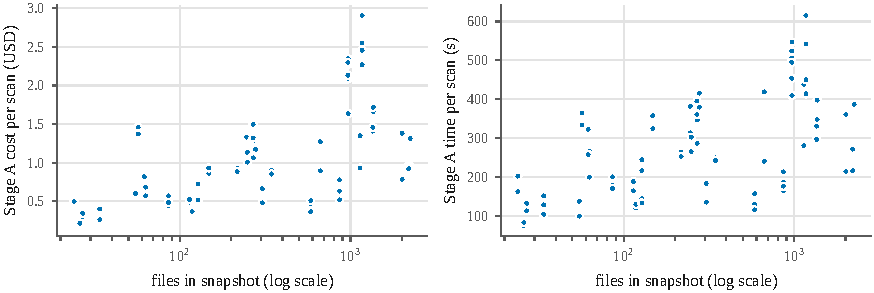
\includegraphics[width=\columnwidth]{fig-cost.pdf}
\caption{Stage A cost and time per scan against the number of files in the
snapshot (82 dev-v4 runs, measured).}
\label{fig:cost}
\end{figure}
